% What "the ring splits the projector" asks for.  Section 5's side condition
% is that a rank-one projection P lying over the ring be P = z z^dagger for a
% vector z ALSO over the ring, and the two halves of that sentence are what a
% reader confuses: P's entries and z's entries are different demands.
%
% LEFT: the outer product, so that "rank one" and "z z^dagger" are one
% picture -- every entry of P is one entry of z times the conjugate of
% another, so the whole matrix is decided by d numbers.
%
% RIGHT: one projector, two rings, two answers.  This is the load-bearing
% panel: P is the SAME matrix in both rows.  What changes is the ring the
% splitting vector is allowed to live in, which is why section 5 is about a
% ring and not about a matrix.
%
% WIDTH. \textwidth is 395.8pt; this is about 370pt.
%
%   make figures                              compiles it
%   \includegraphics{figures/splitting}       includes it
\documentclass[tikz,border=3pt]{standalone}
% ---------------------------------------------------------------------------
% figures/house.tex -- the shared look. Every figure \input's this, so six
% figures look like one hand drew them instead of six.
%
% HOW FIGURES WORK HERE. tikz/pgf is NOT on ACM's production package list, so
% the documents never load it. Each figure is its own standalone document in
% this directory, compiled to a PDF by `make figures`, and pulled into a
% section with
%
%     \begin{figure}
%       \centering
%       \includegraphics{figures/my-figure}
%       \caption{What to LOOK at, not what the figure is of.}
%       \label{fig:my-figure}
%     \end{figure}
%
% Three conventions:
%   * a float sits where it is discussed;
%   * a caption says what to look at, not what the figure is of;
%   * a figure is checked by rendering it and looking, not by a clean compile.
%
% The palette below is the same as the one in preamble.tex. It is repeated
% rather than shared because these are standalone documents that never see the
% paper's preamble, so a colour changed there must be changed here too.
% ---------------------------------------------------------------------------
\usepackage{amsmath}
% The figures build with LuaLaTeX like the documents, so their text is the
% paper's Libertine and their code is the paper's Iosevka.
\usepackage{fontspec}
\setmainfont{LinLibertine_R.otf}[BoldFont=LinLibertine_RB.otf,ItalicFont=LinLibertine_RI.otf,BoldItalicFont=LinLibertine_RBI.otf,Ligatures=TeX]
\setmonofont{Iosevka Custom}[Scale=MatchLowercase,RawFeature={-liga,-calt,-clig,-dlig}]
% Math in the figures is the paper's math: acmart sets Libertinus Math under
% LuaTeX, so the letters on a wire match the letters in the text around it.
\usepackage{unicode-math}
\setmathfont{LibertinusMath-Regular.otf}
\usetikzlibrary{positioning,arrows.meta,fit,backgrounds,calc}

% Blackboard Z, which the documents get from the paper preamble.
% Kept here so a figure never reaches for the paper's preamble.
\newcommand{\Z}{\mathbb{Z}}


\definecolor{ink}{HTML}{16191D}
\definecolor{accent}{HTML}{1F4E79}
\definecolor{accentsoft}{HTML}{E8EEF4}
% accent, accentwarm and accentplum mark the temporary's basis level -- level
% 0, 1, 2 -- wherever a picture or a matrix has to show which branch is which.
\definecolor{accentwarm}{HTML}{9A5B00}
\definecolor{accentplum}{HTML}{8E2F5F}
\definecolor{muted}{HTML}{5B6470}
\definecolor{hairline}{HTML}{C9CFD6}

\tikzset{
  % Every figure inherits this: thin lines, small type, generous air.
  house/.style={
    >={Stealth[length=2.1mm, width=1.6mm]},
    line width=0.5pt,
    node distance=9mm and 15mm,
    every node/.style={font=\small},
  },
  % A thing.
  box/.style={
    draw=ink, line width=0.5pt, rounded corners=1.5pt,
    inner xsep=6pt, inner ysep=4pt, align=center,
  },
  % A thing we are drawing attention to. One per figure, at most.
  boxhi/.style={box, draw=accent, fill=accentsoft, text=ink},
  % A thing that is context, not content.
  boxdim/.style={box, draw=hairline, text=muted},
  % An arrow, and the word on it.
  flow/.style={->, draw=ink},
  flowdim/.style={->, draw=hairline},
  lbl/.style={font=\footnotesize\itshape, text=accent, inner sep=2pt},
  lbldim/.style={font=\footnotesize, text=muted, inner sep=2pt},
  % A dashed grouping rectangle behind a set of nodes.
  group/.style={draw=hairline, dashed, rounded corners=2pt, inner sep=7pt},
}


\tikzset{
  cell/.style={draw=accent, line width=0.6pt, fill=accentsoft,
               minimum size=6.5mm, inner sep=0pt, font=\scriptsize, text=ink},
  vcell/.style={cell, fill=accentwarm!12, draw=accentwarm},
  lb/.style={font=\scriptsize, text=muted, inner sep=1.5pt},
  hot/.style={font=\scriptsize, text=accent, inner sep=1.5pt},
  yes/.style={font=\scriptsize, text=accent},
  no/.style={font=\scriptsize, text=accentplum},
}

\begin{document}
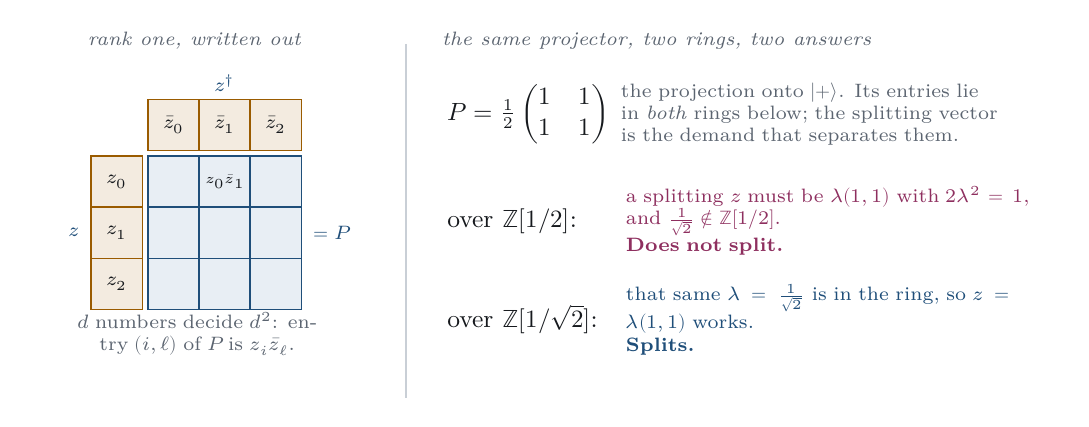
\begin{tikzpicture}[house]

% ------------------------------------------------ LEFT: P = z z^dagger
\node[lb, anchor=south west] at (-1.15,1.62) {\textit{rank one, written out}};

% the row z^dagger, above the grid
\foreach \l in {0,1,2}{
  \pgfmathsetmacro{\xx}{\l*0.65}
  \node[vcell] (zd\l) at (\xx,0.72) {$\bar z_{\l}$};}
% the column z, left of the grid
\foreach \i in {0,1,2}{
  \pgfmathsetmacro{\yy}{-\i*0.65}
  \node[vcell] (zc\i) at (-0.72,\yy) {$z_{\i}$};}
% the product
\foreach \i in {0,1,2}{
  \foreach \l in {0,1,2}{
    \pgfmathsetmacro{\xx}{\l*0.65}
    \pgfmathsetmacro{\yy}{-\i*0.65}
    \node[cell] (p\i\l) at (\xx,\yy) {};}}
\node[font=\tiny, text=ink] at (p01) {$z_{0}\bar z_{1}$};
\node[hot, anchor=south] at (0.65,1.08) {$z^{\dagger}$};
\node[hot, anchor=east] at (-1.14,-0.65) {$z$};
\node[hot, anchor=west] at (1.72,-0.65) {$= P$};
\node[lb, anchor=north, align=center, text width=42mm] at (0.3,-1.6)
  {$d$ numbers decide $d^{2}$: entry $(i,\ell)$ of $P$ is $z_{i}\bar z_{\ell}$.};

% ------------------------------------------------ divider
\draw[draw=hairline] (2.95,1.75) -- (2.95,-2.75);

% ------------------------------------------------ RIGHT: one P, two rings
\node[lb, anchor=south west] at (3.35,1.62)
  {\textit{the same projector, two rings, two answers}};

\node[anchor=west, font=\small, text=ink] at (3.35,0.86)
  {$P = \tfrac12\begin{pmatrix} 1 & 1 \\ 1 & 1\end{pmatrix}$};
\node[lb, anchor=west, align=left, text width=48mm] at (5.62,0.86)
  {the projection onto $|{+}\rangle$. Its entries lie in \emph{both} rings
   below; the splitting vector is the demand that separates them.};

% row 1 -- Z[1/2]
\node[anchor=west, font=\small, text=ink] at (3.35,-0.5) {over $\Z[1/2]$:};
\node[no, anchor=west, align=left, text width=54mm] at (5.62,-0.5)
  {a splitting $z$ must be $\lambda(1,1)$ with $2\lambda^{2} = 1$, and
   $\tfrac{1}{\sqrt2} \notin \Z[1/2]$.\\ \textbf{Does not split.}};

% row 2 -- Z[1/sqrt2]
\node[anchor=west, font=\small, text=ink] at (3.35,-1.75) {over $\Z[1/\sqrt2]$:};
\node[yes, anchor=west, align=left, text width=54mm] at (5.62,-1.75)
  {that same $\lambda = \tfrac{1}{\sqrt2}$ is in the ring, so
   $z = \lambda(1,1)$ works.\\ \textbf{Splits.}};

\end{tikzpicture}
\end{document}
